\section{Additional examples} 
\subsection{The symbolists: use of the macro \tkzcname{includegraphics}}  
\Imacro{includegraphics}

\begin{alterqcm}[lq=8cm,numprop=true,sep]
\AQquestion[pq=2 cm]{Among the three paintings opposite, which is the one painted by \textbf{Gustave Moreau}\vfill}%
{{%
\hfil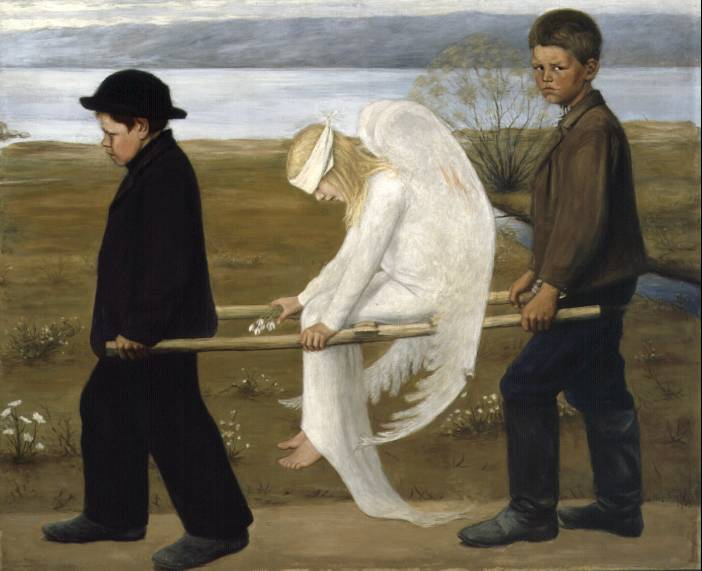
\includegraphics[scale=.20]{The_Wounded_Angel_-_Hugo_Simberg.jpg}\hfil
},{%
\hfil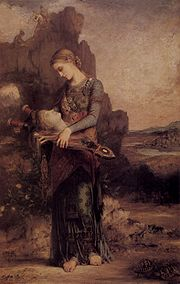
\includegraphics[scale=.4]{180px-Gustave_Moreau_007.jpg}\hfil
},{%
\hfil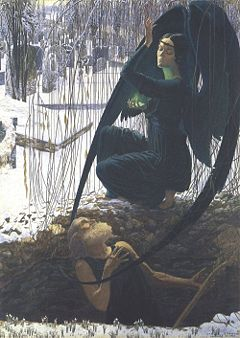
\includegraphics[scale=.4]{240px-Mort_du_fossoyeur.jpg}\hfil}}%
 \AQquestion[pq=1 cm]{The following picture was painted by which of these three painters?\\
\hfil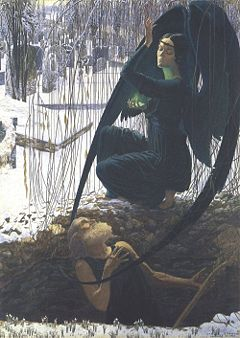
\includegraphics[height=3in]{240px-Mort_du_fossoyeur.jpg}\hfil}%
{{Gustav Klimt},{Carlos Schwabe},{Odilon Redon}}
\end{alterqcm} 

\begin{tkzltxexample}[small]
 \begin{alterqcm}[lq=8cm,numprop=true,sep]
 \AQquestion[pq=2 cm]{Of the three paintings, which is the one painted by \textbf{Gustave Moreau}\vfill}%
 {{%
 \hfil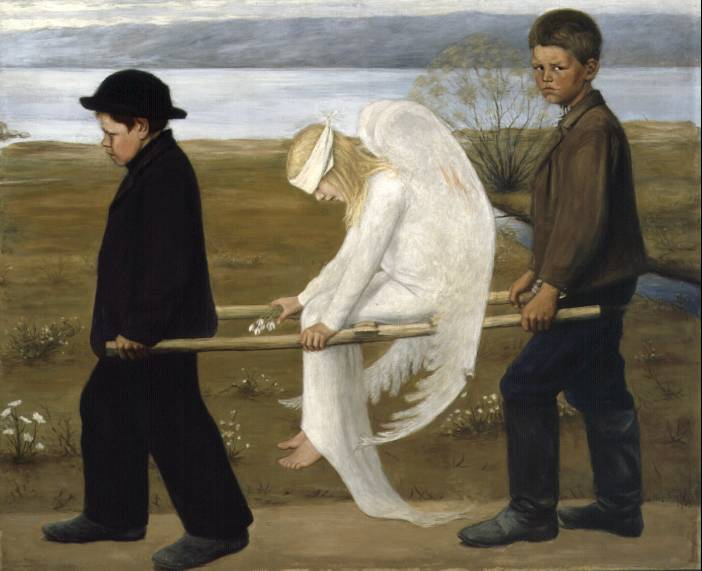
\includegraphics[scale=.25]{The_Wounded_Angel_-_Hugo_Simberg.jpg}\hfil
 },{%
 \hfil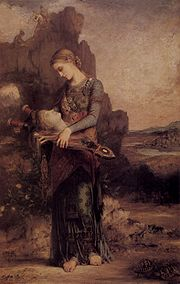
\includegraphics[scale=.5]{180px-Gustave_Moreau_007.jpg}\hfil
 },{%
 \hfil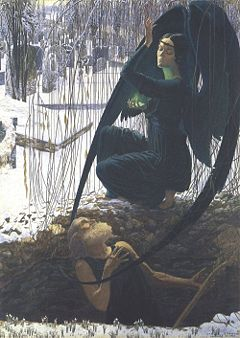
\includegraphics[scale=.4]{240px-Mort_du_fossoyeur.jpg}\hfil}}
  \AQquestion[pq=1 cm]{The following painting, was painted by which of these three painters?\\
 \hfil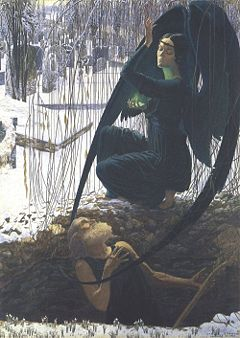
\includegraphics[height=3in]{240px-Mort_du_fossoyeur.jpg}\hfil}%
 {{Gustav Klimt},{Carlos Schwabe},{Odilon Redon}}
 \end{alterqcm} 
\end{tkzltxexample}

\subsection{Using a \tkzname{tikzpicture} environment in a question} 
\Ienv{tikzpicture}

\medskip

\begin{alterqcm}[lq=120mm,pre=true,pq=3mm]
 \AQmessage{\begin{minipage}{15cm}
\vspace*{6pt}   
The three trees given below represent probabilistic situations. %
  The numbers shown on the various arrows are probabilities, and,%.
    in the second level, conditional probabilities. Thus for the given tree %
      in question 1 : $0,35 = P(A)$ and $0,1 =  P_{\text{A}}(E)$.
\vspace*{6pt}    
\end{minipage}  
}
\AQquestion{The probability of event E is equal to : \\
\begin{tikzpicture}[yscale=1.2] 
[parent anchor=east,child anchor=west,grow=east]
\tikzstyle{every node}=[text=Maroon,fill=fondpaille,font=\small]
\tikzstyle{every child}=[level distance=25mm]
\tikzstyle{edge from parent}=[draw,->,thin] 
\tikzstyle{level 2}=[sibling distance=12mm]
\node {}
[grow=right]   
child {node {B}
      child { node {F}
        edge from parent node {$0,5$}}
      child { node {E}
        edge from parent node {$0,5$}
            }
         edge from parent node {$0,65$}
       }
child {node {A}
        child { node {F}
          edge from parentnode {$0,9$}}
        child { node {E}
          edge from parent node {$0,1$}}
      edge from parent node {$0,35$}
      };
\end{tikzpicture}}
{{$0,5$},%
{$0,1$},%
{$0,6$},%
{$0,36$}}
\end{alterqcm} 

\begin{tkzltxexample}[small]
 \begin{alterqcm}[lq=120mm,pre=true,pq=3mm]
  \AQmessage{The three trees given below represent probabilistic situations.
   The numbers shown on the different arrows are probabilities, and,
   in the second level, conditional probabilities. Thus for the given tree 
   in question 1: $0,35 = P(A)$ and $0,1 =  P_{\text{A}}(E)$.}
 \AQquestion{The probability of event E is equal to : \\
 \begin{tikzpicture} 
 ...
 \end{tikzpicture}}
 {{$0,5$},%
 {$0,1$},%
 {$0,6$},%
 {$0,36$}}
 \end{alterqcm} 
\end{tkzltxexample}

\begin{tkzexample}[vbox]
\begin{alterqcm}[lq=8cm,numprop=true,sep]
\AQquestion{Among the figures opposite, indicate the one that is a rhombus. :}
{{\hspace{1cm}  \begin{minipage}{5cm} 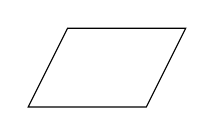
\begin{tikzpicture} 
  \draw (0,0)--(1.5,0)--(2,1)--(.5,1)--cycle; 
\end{tikzpicture} \end{minipage}},
{\hspace{1cm}  \begin{minipage}{5cm} 
\begin{tikzpicture}
   \draw[rotate=30] (0,0) rectangle (1.5,1); \end{tikzpicture} \end{minipage}},
{\hspace{1cm}  \begin{minipage}{5cm} 
\begin{tikzpicture}
   \draw (0,0) rectangle (1,1); \end{tikzpicture} \end{minipage} }}
\end{alterqcm} 
\end{tkzexample}

\subsection{Use of a \tkzname{array} environment in the proposals} 
\Ienv{array}

It is possible to use tables and other structures in the question code or proposals. An example is shown below:

\medskip


\begin{tkzexample}[vbox]
\begin{alterqcm}[lq=88mm,symb=$\Box$]
\AQquestion{The couple $(1~;~-1)$ is a solution of }
{%
{$ \left\lbrace
\begin{array}{ll}
 0,75a + 0,5b &= 0,25 \\
 0,25a + 0,5b &=-0,25
\end{array}\right.$},
{$ \left\{
\begin{array}{ll}
 a &=  0,75a +0,5b \\
 b &=  0,25a +0,5b
\end{array}\right.$},
{$ \left\lbrace
\begin{array}{ll}
 0,75a - 0,5b &= 0,25 \\
 0,5a + 0,25b &=-0,25
\end{array}\right.$}
}
\end{alterqcm}\end{tkzexample}  


\subsection{Use of code \tkzname{verbatim} in questions and proposals} 
\Ienv{verbatim}

Here is an example from Pascal Bertolino. It is preferable to use as Pascal did the macro \tkzcname{texttt}, otherwise avoid the use of the mode 
|verbatim|. We will see on the next page how to proceed if this mode is really necessary.

\begin{alterqcm}[lq=80mm,title=false,long] 

%--------------------------------------------------------------
\AQquestion{What was the precursor language of the C language?}
{{Fortran},
 {Language B},
 {Basic}}

%--------------------------------------------------------------
\verbdef\argprop|int a = 3 ^ 4 ;|
\AQquestion{\argprop}
{{raises 3 to the power of 4},
 {makes an exclusive OR between 3 and 4},
 {is not a C}}

%--------------------------------------------------------------
\AQquestion{What is the correct syntax to shift the integer 8 bits to the left? \texttt{a} ?}
{{\texttt{b = lshift(a, 8) ;}},
 {\texttt{b = 8 << a ;}},
 {\texttt{b = a << 8 ;}}}
%--------------------------------------------------------------
\verbdef\argprop|{ printf ("hello") ; return 0 ; \}|
\AQquestion{The complete program:	\\
\texttt{int main() \\
~~\argprop}}
{{displays \texttt{hello}},
 {gives an error to the compilation},
 {gives an error in execution}}
%--------------------------------------------------------------
\verbdef\arg|float tab[10]|
\verbdef\propa|*tab|\global\let\propa\propa
\verbdef\propb|&tab|\global\let\propb\propb
\verbdef\propc|tab|\global\let\propc\propc
\AQquestion{Let's say the declaration \arg ; \\The first real in the table is \ldots}
{{\propa},
 {\propb},
 {\propc}}

%--------------------------------------------------------------
\AQquestion{The line \texttt{printf("\%c", argv[2][0]) ;}
 of \texttt{main} of  \texttt{monProg} run like this : 
\texttt{monProg parametre }}
{{displays \texttt{p}},
 {displays nothing},
 {can cause a crash}}
%--------------------------------------------------------------
\AQquestion{What is the memory size of a \texttt{long int} ?}
{{4 octets},
 {8 octets},
 {ça dépend \ldots}}
%--------------------------------------------------------------
\AQquestion{Following the declaration \texttt{int * i} ;}
{{\texttt{*i} is an address},
 {\texttt{*i} is an integer},
 {\texttt{*i} is a pointer}}
%--------------------------------------------------------------
\AQquestion{One of the following choices is not a standard C library}
{{\texttt{stdlib}},
 {\texttt{stdin}},
 {\texttt{math}}}

\end{alterqcm}

\medskip
Let's look at the source code

the simplest way is often to use the command \tkzcname{texttt}

\begin{tkzexample}[code only]
 \AQquestion{Following the declaration \texttt{int * i} ;}
 {{\texttt{*i} is an address},
 {\texttt{*i} is an integer},
 {\texttt{*i} is a pointer}}
\end{tkzexample}

\begin{tkzexample}[code only]
\AQquestion{The line \texttt{printf("\%c", argv[2][0]) ;}
 of \texttt{main} of  \texttt{monProg} run like this : 
\texttt{monProg parametre }}
{{displays \texttt{p}},
 {displays nothing},
 {can cause a crash}}
\end{tkzexample}

Alternatively, we can load the \tkzname{verbdef} package:
\tkzNamePack{verbdef}

\tkzcname{usepackage\{verbdef\}}

\begin{tkzexample}[code only]
 \verbdef\argprop|int a = 3 ^ 4 ;|
 \AQquestion{\argprop}
 {{raises 3 to the power of 4},
 {does an exclusive OR between 3 and 4},
  {is not a C-instruction}}
\end{tkzexample}

More than one variable may be required:

\begin{tkzexample}[code only]
 \verbdef\arg|float tab[10]|
 \verbdef\propa|*tab|\global\let\propa\propa
 \verbdef\propb|&tab|\global\let\propb\propb
 \verbdef\propc|tab|\global\let\propc\propc
 \AQquestion{Either the declaration  \arg ; \\
 The first real in the table is \ldots}
 {{\propa},
  {\propb},
  {\propc}}
\end{tkzexample}

\endinput